
%%% Local Variables: 
%%% mode: latex
%%% TeX-master: t
%%% End: 

\chapter{环结构在扇贝图像识别中的应用}
\label{cha:intro}

\renewcommand\arraystretch{1}

\section{扇贝图像识别研究现状}
\label{}

人们对海洋食品的需求不断增长,以海洋捕捞为主的渔业逐步转变为以海水养殖为主。近些年来,我国的海水养殖业得到了迅猛发展,在北方,扇贝已成为一个重要的经济贝类养殖品种。但养殖的自动化水平还与一些国家有较大差距,需要进一步进行研究与应用,生产养殖的自动化技术的研究和应用已引起广泛重视\cite{zhucongrong}。

扇贝属于软体体动物门、双壳纲、翼形亚纲、珍珠贝目、扇贝科、扇贝属。中国的常见的养殖种类:栉孔扇贝、海湾扇贝、虾夷扇贝、华贵栉孔扇贝。在扇贝的养殖过程中,需要按扇贝的种类及大小进行分类,通常情况下,扇贝的分类工作依赖于工人的辛勤劳动,这种方法不仅费时而且需要检测人员具有一定的经验。使用机械进行筛选容易使扇贝受到碰撞,边缘受到损伤,造成扇贝死亡的情况。

通过计算机视觉技术来检测扇贝,具有实时、高效、无损坏等特点,可以替代传统的人工检测的方式。国内外很多学者都针对扇贝的分类问题采用计算机视觉技术进行了相关研究。

Mikamip\cite{mikamip}研究了扇贝的外部形态特征,开发了机械化分类技术,2006年,他实现了基于图像处理技术的非接触式扇贝分类技术。林艾光\cite{linaiguang}等人研究了测量扇贝大小的方法,建立了数学模型来研究扇贝贝壳面积与扇贝壳长之间的关系,从而实现了根据大小来识别扇贝的目的。郭常有\cite{guochangyou}利用改进的OPTA算法与边界追踪算法提取扇贝图像的边界,通过计算扇贝图像边界点相对距离的最大值来识别扇贝的尺寸。杨晓光\cite{yangxiaoguang}等人结合大津法与YCRCB颜色空间来分割扇贝图像,完成了对扇贝的检测和测量。魏洪磊\cite{weihonglei}等人建立了一个模糊识别系统,实现了陕北的识别和分类。首先用Canny算子提取图像边缘,边缘之间的均值与距离方差、扇贝贝壳中心点及种类作为系统的输入和输出。杨眉\cite{yangmei}等人提出里基于神经网络的识别系统。用Canny算子检测扇贝边缘,并且得到边缘像素的坐标,利用训练好的BP神经网络,通过均值和方差的距离来作为分类特征来进行识别。

然而,这些方法很大程度上都取决于扇贝的边缘,如果拍摄角度或焦距产生变化,或者扇贝的边缘受到损坏,可能会导致这些方法失效。另外,这些方法只能进行大小或种类的分类或识别,而无法识别出扇贝个体。

基于此,我们提出了使用环结构特征来对扇贝个体进行识别。我们知道,每个扇贝都有自己独特的贝壳纹理,就如每个人的指纹一样可以作为独特的特征来区分。扇贝的生长纹与放射肋是扇贝纹理的显著特征,他们之间通常相交形成稳定的环结构,无论拍摄角度怎样变化,环结构都可作为一种显著且稳定的特征来用作识别。图\ref{fig:scallop}给出了三幅扇贝图像的例子,每个扇贝的纹理都有很大程度的不同,蓝色的线表示生长纹,红色的线代表放射肋,它们相交产生环结构。我们通过分割及骨架化提取出环结构,再用通过把环结构描述成特征向量,即可通过特征向量的匹配来识别出扇贝个体。

在扇贝养殖过程中,不同扇贝所需的生长环境是不同的,例如水温、盐度等因素,通过研究扇贝生长纹,也可帮助估算扇贝年龄\cite{hurley}与计算扇贝生长速率\cite{david},以此来了解扇贝在何种环境下生长最迅速,或在何种环境下容易导致扇贝死亡,这对我国的扇贝养殖事业也有很大的推动作用,同时,年龄的估算也可避免过度捕捞,便于渔场的有效管理。

\begin{figure}
\centering
  \begin{minipage}[b]{0.3\textwidth} 
      \centering 
      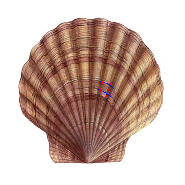
\includegraphics[width=4cm]{chap04/11}
        \centerline{(a)}\medskip
    \end{minipage}
  \begin{minipage}[b]{0.3\textwidth}
    \centering
    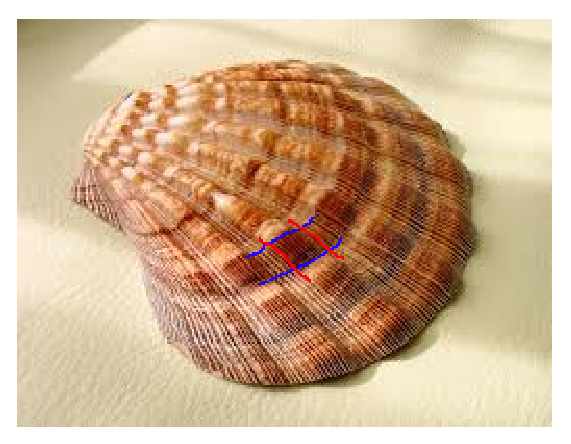
\includegraphics[width=5cm]{chap04/20}
      \centerline{(b)}\medskip
  \end{minipage}
  \begin{minipage}[b]{0.3\textwidth}
    \centering
    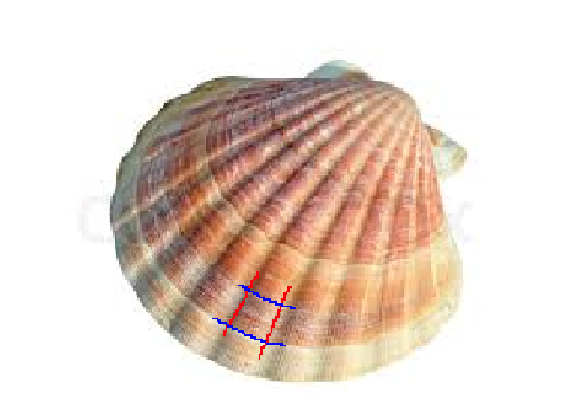
\includegraphics[width=6cm]{chap04/28}
      \centerline{(c)}\medskip
  \end{minipage}
\caption{扇贝纹理及环结构}
\label{fig:scallop}
\end{figure}



图\ref{fig:scallop-framework}所示为扇贝图像识别的基本流程图。参考图像库中的扇贝图像与待识别图像库中的扇贝需要进行图像分割与骨架化,从而提取出扇贝生长纹和放射肋,我们采用基于广度优先策略的环结构检测算法检测环结构,然后用组成环结构的分叉点的分支角度及纹路的长度来把环结构描述为特征向量。取待识别图像库中一幅图像的特征向量与参考图像中的所有特征向量进行匹配,找到最相似的环结构对,并判断这对特征对是否相对应于同一个扇贝,若是,则说明识别成功,否则,则识别失败。


\begin{figure}
  \centering
  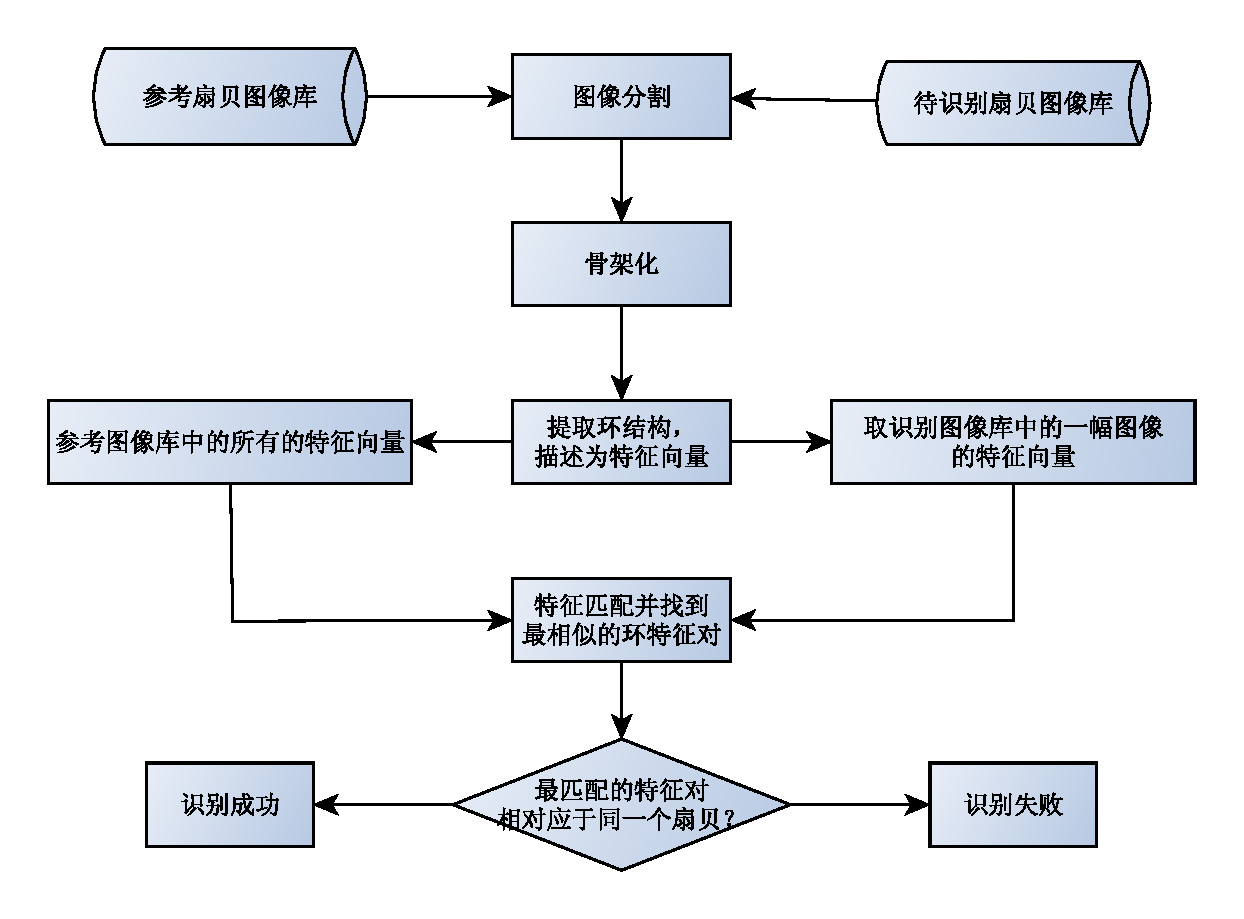
\includegraphics[width=0.8\textwidth]{chap04/scallop-framework}
  \caption{扇贝图像识别}
  \label{fig:scallop-framework}
\end{figure}
\section{扇贝图像数据库构建}
\label{}
由于没有公开的用于扇贝识别的图像数据库,我们从网络上采集了一部分扇贝图像数据作为实验对象。图\ref{fig:scallop}所示为几个从网络中采集的扇贝图像的例子。

在实际的扇贝识别过程中,有时会出现扇贝平移、旋转、遮挡,焦距变化等情况,为了证明我们的算法能够在这些情况下具有鲁棒性,把从网络搜集的扇贝图像直接作为参考图像库,共包含10幅不同扇贝个体的图像。待识别图像库中的扇贝图像是参考图像库中的图像经过旋转、缩放及部分遮挡的处理得到的,故待识别图像库中共包含30幅图像。扇贝识别即是在参考图像库中找出与待识别图像相同的扇贝个体。如图\ref{fig:process},是扇贝原图及经过放大、遮盖、旋转的扇贝图像,原图则放入参考图像库,经过处理的扇贝图像则放入待识别图像库,若能在参考图像中检测到与待识别图像相对应的原图,则说明识别成功。

\begin{figure}
\centering
  \begin{minipage}[b]{0.48\textwidth} 
      \centering 
      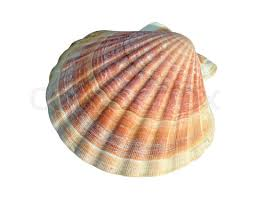
\includegraphics[width=5cm]{chap04/28-ori}
        \centerline{(a)原图}\medskip
    \end{minipage}
  \begin{minipage}[b]{0.48\textwidth}
    \centering
    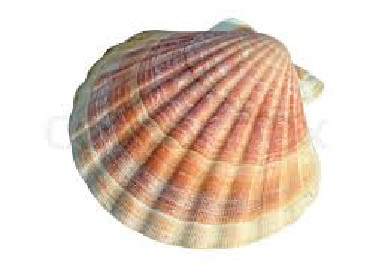
\includegraphics[width=6cm]{chap04/28-da}
      \centerline{(b)放大图}\medskip
    \end{minipage}
  \begin{minipage}[b]{0.48\textwidth} 
      \centering 
      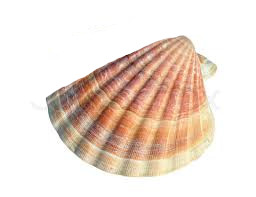
\includegraphics[width=5cm]{chap04/28-qu}
        \centerline{(c)遮盖图}\medskip
    \end{minipage}
  \begin{minipage}[b]{0.48\textwidth}
    \centering
    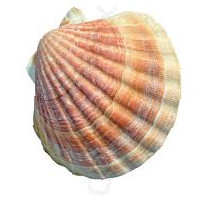
\includegraphics[width=4cm]{chap04/28-zhuan}
      \centerline{(d)旋转图}\medskip
  \end{minipage}
\caption{扇贝参考图像与待识别图像}
\label{fig:process}
\end{figure}

参考图像库中的图像与待识别图像库中的图像都要经过图像分割与图像骨架化处理,以得到二值化的具有单像素宽的扇贝纹理,以为提取环结构做好准备。我们采用基于偏微分方程的多尺度分割方法与轮廓修剪骨架提取方法来对两个图像库中的图像进行处理,如图\ref{fig:seg-skel}所示为一个扇贝分割与骨架化的例子。从图中可以看出,经过分割与骨架化后的图像能很好的提取出原图像中扇贝的生长纹与放射肋。

\begin{figure}
\centering
  \begin{minipage}[b]{0.48\textwidth} 
      \centering 
      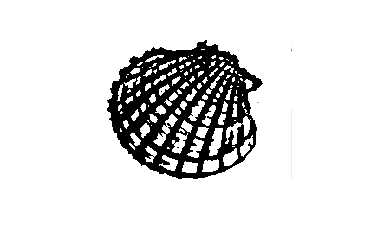
\includegraphics[width=6cm]{chap04/28-suoxiao}
        \centerline{(a)放大分割图}\medskip
    \end{minipage}
  \begin{minipage}[b]{0.48\textwidth}
    \centering
    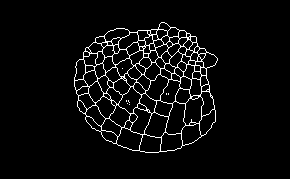
\includegraphics[width=5cm]{chap04/28-suoxiao-skel}
      \centerline{(b)放大骨架化图}\medskip
    \end{minipage}
  \begin{minipage}[b]{0.48\textwidth} 
      \centering 
      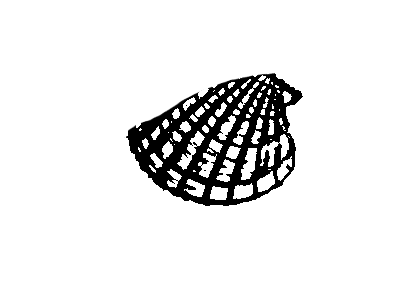
\includegraphics[width=5cm]{chap04/28-zhegai}
        \centerline{(c)遮盖分割图}\medskip
    \end{minipage}
  \begin{minipage}[b]{0.48\textwidth}
    \centering
    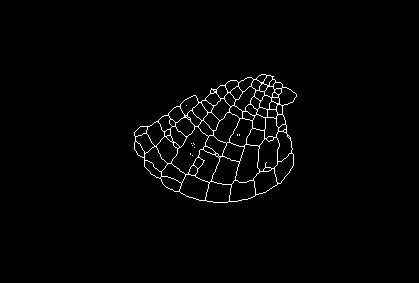
\includegraphics[width=5cm]{chap04/28-zhegai-skel}
      \centerline{(d)遮盖骨架化图}\medskip
  \end{minipage}
  \begin{minipage}[b]{0.48\textwidth} 
      \centering 
      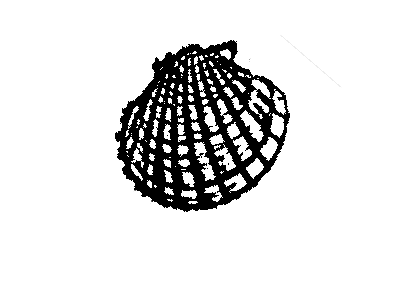
\includegraphics[width=5cm]{chap04/28-xuanzhuan}
        \centerline{(e)旋转分割图}\medskip
    \end{minipage}
  \begin{minipage}[b]{0.48\textwidth}
    \centering
    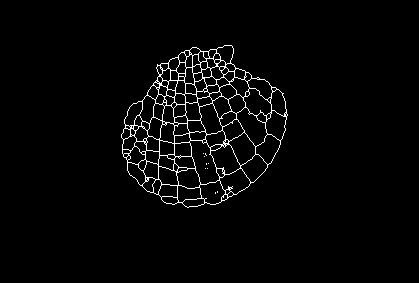
\includegraphics[width=5cm]{chap04/28-xuanzhuan-skel}
      \centerline{(f)旋转骨架化图}\medskip
  \end{minipage}
\caption{扇贝图像分割与骨架化}
\label{fig:seg-skel}
\end{figure}

在扇贝贝壳图像中检测环结构是完成识别的关键的一步。只有成功的精准的检测到扇贝图像中的环结构,才能为扇贝识别做好准备。从分割图中可以看出,环结构大都是由三点、四点、五点环组成的,我们采用我们提出的环结构检测算法来检测环结构,图\ref{fig:scallop-cycle}是环结构检测的例子。从图中可以看出,检测到的环结构特征与实际扇贝贝壳纹理特征有很好的贴合。

\begin{figure}
\centering
  \begin{minipage}[b]{0.48\textwidth} 
      \centering 
      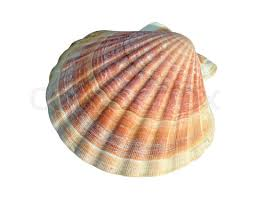
\includegraphics[width=5cm]{chap04/28-ori}
        \centerline{(a)原图}\medskip
    \end{minipage}
  \begin{minipage}[b]{0.48\textwidth}
    \centering
    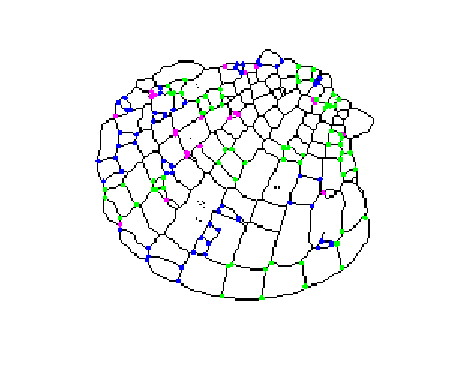
\includegraphics[width=5cm]{chap04/scallop-cycle1}
      \centerline{(b)环结构}\medskip
    \end{minipage}
\caption{扇贝参考图像与待识别图像中的环结构}
\label{fig:scallop-cycle}
\end{figure}


\section{环结构匹配与扇贝图像识别}
\label{}

检测环结构后,我们采用分支角度与分支长度来把环结构描述成为归一化的特征向量,由此,扇贝图像识别问题就转化为特征向量的匹配问题。

我们采用相似性度量准则来对待识别图像库中的一幅图像的特征向量与标准图像库中所有扇贝图像你的特征向量进行匹配,得到最匹配的环结构特征对。由于组成环结构的分叉点个数不同,分支角度与分支长度的个数不同,则不同的环的特征向量的长度也会有所不同。特征匹配只在相同类型的环之间进行,由此,我们可以得到最匹配的三对环结构特征。若最匹配的特征对相对应于同一个扇贝的图像,则说明识别成功,否则,则识别失败。如图\ref{fig:recognition},表示标准图像库中的骨架化图像与待识别库中的骨架化图像,它们都来自于同一个扇贝,图中彩色标记的环结构为找到的匹配的环结构,可以看出,这些匹配的环结构都是正确的。

\begin{figure}
\centering
  \begin{minipage}[b]{0.48\textwidth} 
      \centering 
      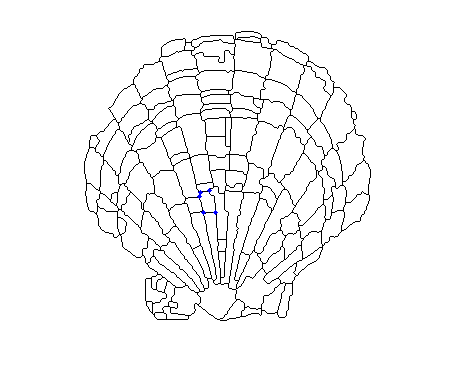
\includegraphics[width=6cm]{chap04/suoxiao-yuantu}
        \centerline{(a)原图}\medskip
    \end{minipage}
  \begin{minipage}[b]{0.48\textwidth}
    \centering
    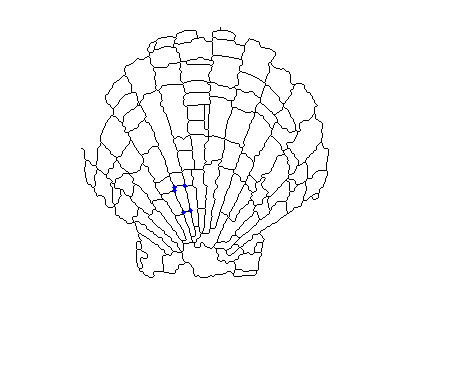
\includegraphics[width=6cm]{chap04/suoxiao}
      \centerline{(b)缩小后图像}\medskip
    \end{minipage}
  \begin{minipage}[b]{0.48\textwidth} 
      \centering 
      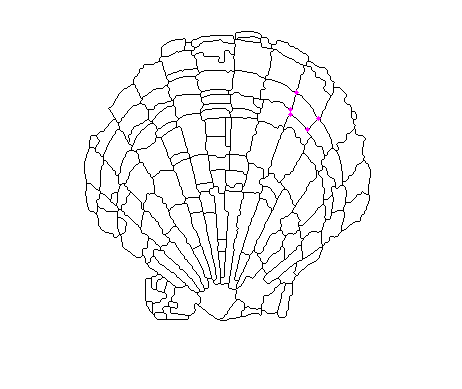
\includegraphics[width=6cm]{chap04/zhegai-yuantu}
        \centerline{(a)原图}\medskip
    \end{minipage}
  \begin{minipage}[b]{0.48\textwidth}
    \centering
    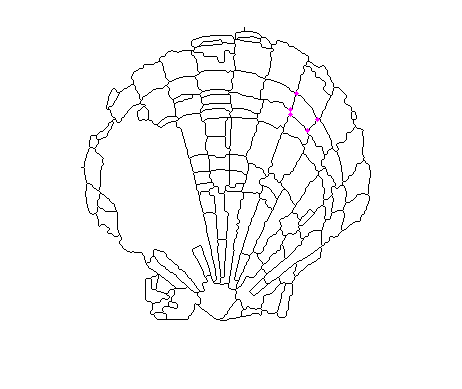
\includegraphics[width=6cm]{chap04/zhegai}
      \centerline{(b)遮盖后图像}\medskip
    \end{minipage}
  \begin{minipage}[b]{0.48\textwidth} 
      \centering 
      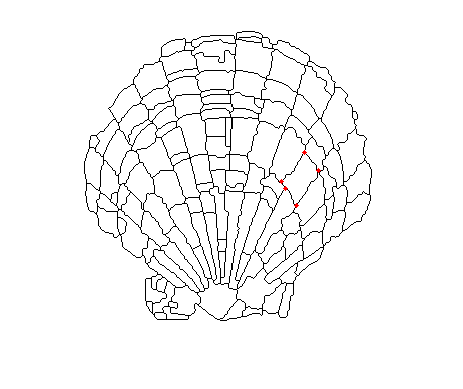
\includegraphics[width=6cm]{chap04/xuanzhuan-yuantu}
        \centerline{(a)原图}\medskip
    \end{minipage}
  \begin{minipage}[b]{0.48\textwidth}
    \centering
    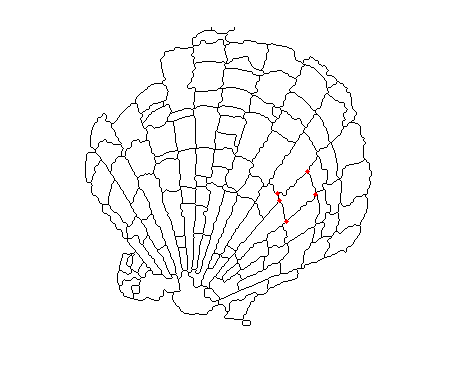
\includegraphics[width=6cm]{chap04/xuanzhuan}
      \centerline{(b)旋转后图像}\medskip
    \end{minipage}
\caption{扇贝参考图像与待识别图像中匹配的环结构}
\label{fig:recognition}
\end{figure}

通过网络搜索的扇贝图像制作的数据库,进行了扇贝识别实验,成功率分别为83.3\%,详见表\ref{tab:recognition}。由表中可以看到,由于旋转和尺度变化造成的识别失败的情况较多,这是因为在对图像进行旋转和尺度变化时进行了插值运算,这样就可能改变原图像中的环结构特征,从而找不到最匹配的环结构,导致了匹配的失败。
\begin{table}
\caption{扇贝识别结果}
\centering
\begin{tabular}{p{1cm}<{\centering}p{1cm}<{\centering}p{1cm}<{\centering}p{1cm}<{\centering}}
  \hline
  No. & 旋转 & 遮盖 & 尺度\\
  \hline
  \rowcolor{gray!50}
  1 & $\surd$  & $\surd$     & $\surd$ \\
  2 & $\surd$  & $\surd$     & $\surd$ \\
  \rowcolor{gray!50}
  3 & $\times$  & $\surd$  & $\surd$\\
  4 & $\surd$  & $\surd$  & $\surd$ \\
  \rowcolor{gray!50}
  5 & $\surd$     & $\surd$     & $\times$\\
  6 & $\surd$      & $\surd$      & $\surd$\\
  \rowcolor{gray!50}
  7 & $\surd$  & $\times$      & $\surd$  \\
  8 & $\times$  & $\surd$  & $\surd$ \\
  \rowcolor{gray!50}
  9 & $\surd$ & $\surd$  & $\surd$\\
  10 & $\surd$  & $\surd$  & $\times$ \\
  \hline
\end{tabular}
\label{tab:recognition}
\end{table}

\section{本章小节}
\label{}
本章实现了基于环结构特征的扇贝图像识别。在本章中主要介绍如何把环结构特征用于扇贝图像识别上。构建了扇贝图像识别图像库,即包括扇贝标准图像库与待识别图像库,用基于广度优先策略的环结构检测算法来检测环结构并把环结构描述成归一化的特征向量。通过用相似性度量来找到最匹配的环结构特征对,相对应的原图像则是识别结果,通过实验验证了用环结构来进行扇贝图像识别的有效性。

